\documentclass[11pt]{article}
\usepackage[top=0.20in, bottom=.20in, left=0.5in, right=0.5in]{geometry}
\renewcommand{\baselinestretch}{1.1}
\usepackage{graphicx}
\usepackage{natbib}
\usepackage{amsmath}
\usepackage{multicol}
\usepackage{tcolorbox}
\usepackage{caption}
\usepackage{todonotes}
\usepackage[font={sf,footnotesize}]{caption}
\usepackage{hyperref}
\newcommand{\llabel}[1]{\hypertarget{lintarget:#1}{}\linelabel{lin:#1}}

\usepackage{lineno}
\renewcommand\linenumberfont{\normalfont\tiny\color{gray}}


\bibliographystyle{besjournals}

\begin{document}

% \title{Closing the gap between statistical and scientific workflows for improved forecasts in ecology} 
\title{\large Closing the gap between statistical and scientific workflows for improved forecasts in ecology\\Supplementary material}
\date{}
\author{\small Victor Van der Meersch$^{1*}$, James Regetz$^{2}$, T. Jonathan Davies$^{1,3}$ \& EM Wolkovich$^{1}$}
\maketitle
{\footnotesize \noindent $^{1}$ Forest and Conservation Sciences, University of British Columbia, Vancouver, BC V6T 1Z4, Canada\\
$^{2}$ National Center for Ecological Analysis and Synthesis, 1021 Anacapa St, Santa Barbara, CA 93101, United States\\
$^{3}$ Botany, University of British Columbia, Vancouver, BC V6T 1Z4, Canada \\
$^{*}$ \url{mailto:victor.vandermeersch@ubc.ca}

\renewcommand{\thefigure}{S\arabic{figure}}

\begin{figure}[b]
	\centering
    \vspace*{-20cm}
	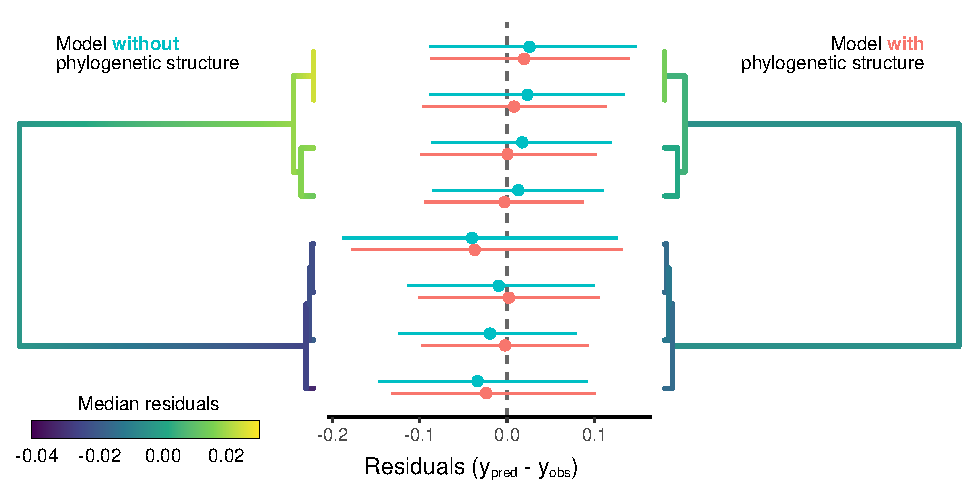
\includegraphics{../figures/retrodic/retrodictive_check.pdf}
	\caption{A simple illustration of a retrodictive check to highlight a missing structure in a model. Here, we consider ``observations'' simulated from a linear regression model ($y_\text{obs}$), for 8 different species. The species-specific intercepts and slopes are simulated with a phylogenetic structure, i.e. the correlation between two species-specific parameters is proportional to the amount of evolutionary history (as defined by a simulated phylogenetic tree, shown in the left and right parts of the figure) shared by the two species. As a first approach, we use a model with partial pooling on the intercepts and the slopes---assuming no correlation structure---to fit the data. We can simulate data from the fitted model ($y_\text{pred}$), and compare the retrodictions to the observations---i.e. doing a retrodictive check. The check has to be tailored in regard to our research question and our domain expertise: here, we might believe that some species are more closely related than others, and we want to visually check whether we find some apparent distinctions between species groups (``clades''). In the left part of the figure, we find some (small) symptoms of a missing group structure: the upper clade residuals tend to have a positive bias, while the lower clade ones have a negative bias. This retrodictive check indicates that we could refine our model, using the same phylogenetic correlation structure that we used to simulate data (i.e. the same phylogenetic tree). With this new refined model, we can perform a new retrodictive check (right part of the figure): the difference of residual biases between the two distinct clades now appears smaller. \\
	Interestingly, when looking at the interquartile range of these residuals (middle part of the figure), both models (with and without phylogenetic structure) seem less distinct. This illustrates that we may need to spend more time to build a more adapted retrodictive check. The addition of correlation structure in our second model should indeed mostly result in a reduction in species-specific parameter uncertainty rather than an important shift to the $y_\text{pred}$ themselves. One might need to develop a smarter check, for example looking at empirical covariance between species two by two.}
	\label{fig:modeldata}
	\vspace*{2cm}
\end{figure}

\end{document}
